% Chapter 1

\chapter{Motivations and Problem Statement (Rooshan Khan)} % Write in your own chapter title
\label{Chapter1}
\lhead{Chapter 1. \emph{Motivations and Problem Statement}} % Write in your own chapter title to set the page header

Pre-trained models like BERT (Bidirectional Encoder Representations from Transformers), presented by Devlin and colleagues in their work \textit{BERT: Pre-training of Deep Bidirectional Transformers for Language Understanding}~\cite{devlin2018bert}, have transformed natural language processing by setting new benchmarks across numerous downstream tasks. However, despite its success, the BERT model is known to suffer from issues related to \textbf{robustness}—its ability to maintain consistent performance when exposed to challenging, noisy, or perturbed inputs. Furthermore, typical fine-tuning strategies often lead to large, unstable updates, making the model prone to \textbf{overfitting}, especially when training on limited data.

In our work, we aim to improve the robustness and generalizability of the BERT model. Unlike traditional approaches where separate BERT models are fine-tuned independently for each downstream task, we adopt a \textbf{sequential fine-tuning strategy} in which a single BERT model is progressively fine-tuned across multiple tasks. Specifically, the same BERT model is trained first on paraphrase detection (QQP), then on semantic textual similarity (STS-B), and finally on sentiment analysis (SST-5). This approach allows for the transfer of useful knowledge between tasks while keeping the model size compact.

We propose a robust fine-tuning framework that integrates the following components:
\begin{itemize}
    \item \textbf{Smoothness-Inducing Adversarial Regularization:} Enhances model robustness by training it to resist small perturbations in the input space.\cite{jiang2019smart}
    \item \textbf{Bregman Proximal Point Optimization:} Prevents large and unstable parameter updates during fine-tuning, ensuring smoother convergence and reducing overfitting.\cite{jiang2019smart}
    % \item \textbf{Contrastive Learning:} Optimizes sentence embeddings by encouraging semantically similar sentence pairs to be closer in the embedding space, and dissimilar pairs to be farther apart.\cite{gao2021simcse}
    \item \textbf{Contrastive Learning:} Enhances sentence representations by pulling embeddings of semantically related sentence pairs closer together, while pushing apart those of unrelated pairs within the embedding space.

\end{itemize}

We also adopt the \textbf{Siamese Sentence-BERT (SBERT)} architecture to create meaningful sentence embeddings that capture semantic similarity, enabling efficient comparison of sentence pairs.\cite{reimers2019sentence}

Our experiments use the \textbf{BERT-Base model} due to its manageable size. However, the proposed techniques can be extended to larger BERT variants, such as BERT-Large, in future work.

Table~\ref{tasks_ratings1} presents the performance of the baseline BERT model on these tasks.
\begin{table}[h]
    \centering
    \begin{tabular}{|c|c|}
        \hline
        Tasks & Accuracies(1st 2) and Pearson Correlation (last) \\ 
        \hline
        Sentiment Analysis & 0.144 \\ 
        Paraphrase Detection & 0.369 \\ 
        Semantic Textual Similarity & -0.009 \\
        \hline
    \end{tabular}
    \caption{Tasks and Ratings for simple BERT model without finetuning}
    \label{tasks_ratings1}
\end{table}

\textbf{Motivation:} Looking at Table~\ref{tasks_ratings1}, we recognized the need for fine-tuning. We wanted to investigate how fine-tuning the same model for different tasks affects its performance on those tasks—specifically, whether it improves performance on individual tasks or has the opposite effect. We explored this question using our selected tasks. Our experiments showed a slight improvement in accuracy, but it was not significant. Hence, fine-tuning alone is not sufficient. It needs to be combined with additional techniques from research papers, which we discuss in the following sections.

% \begin{table}[h]
%     \centering
%     \begin{tabular}{|c|c|}
%         \hline
%         Tasks & Accuracies(1st 2) and Pearson Correlation (last) \\ 
%         \hline
%         Semantic Textual Similarity(20 epochs) & -0.039 \\
%         Paraphrase Detection(1 epoch) & 0.766 \\
%         Sentiment Analysis(10 epochs) & 0.523 \\
%         \hline
%     \end{tabular}
%     \caption{Tasks and Ratings for multitask fine-tuned BERT model.}
%     \label{tasks_ratings2}
% \end{table}

% Hence, fine-tuning alone is not sufficient. It needs to be combined with additional techniques from research papers, which we discuss in the following sections.
% \section{Research Papers Read}
% In our research, we have studied several key papers in the field of Natural Language Processing (NLP) to gain insights into pretraining, fine-tuning strategies, and sentence embeddings. Notably, we have reviewed \textit{BERT: Pre-training of Deep Bidirectional Transformers for Language Understanding} by Devlin et al. \cite{devlin2018bert}, \textit{SimCSE: Simple Contrastive Learning of Sentence Embeddings} by Gao et al. \cite{gao2021simcse}, \textit{How to Fine-Tune BERT for Text Classification?} by Sun et al. \cite{sun2019fine}, \textit{Sentence-BERT: Sentence Embeddings using Siamese BERT-Networks} by Reimers and Gurevych \cite{reimers2019sentence}, and \textit{SMART: Robust and Efficient Fine-Tuning for Pre-trained Natural Language Models through Principled Regularized Optimization} by Jiang et al. \cite{jiang2019smart}.

% \textbf{The aim of research paper 1(\textit{SMART: Robust and Efficient Fine-Tuning for Pre-trained Natural Language Models through Principled Regularized Optimization} by Jiang et al. \cite{jiang2019smart}):}

% Aggressive fine-tuning often causes fine tuned model to overfit the training data of downstream tasks and fail to generalize to unseen data. To address this issue a new learning framework was proposed in this paper to obtain better generalization performance. The proposed framework contains:
% \begin{itemize}
%     \item Smoothness inducing adversarial regularization which effectively manages the complexity of the model. With such regularization a small perturbation to the input does not change the output of the model much.
%     \item Bregmann Proximal Point Optimization methods introduce a trust-region-type regularization at each iteration, and then update the model only within a small neighborhood of the previous iterate. Therefore, they can effectively prevent aggressive updating and stabilize the fine-tuning process.
% \end{itemize}

% \textbf{The aim of research paper 2(\textit{Sentence-BERT: Sentence Embeddings using Siamese BERT-Networks} by Reimers and Gurevych \cite{reimers2019sentence}:}

% Traditional BERT embeddings are not optimized for sentence similarity tasks. This paper introduces architecture Sentence-BERT (SBERT) that uses Siamese network to generate meaningful sentence embeddings to improve accuracy and pearson correlation coefficient for paraphrase detection and Semantic Textual Similarity tasks respectively. Cosine Similarity is used to improve accuracies of NLP tasks involving sentence pairs.
% SBERT adds a pooling operation to the output of BERT to derive a fixed sized sentence embedding. We will experiment with three pooling strategies: Using the output of the CLS-token, computing the mean of all output vectors (MEAN strategy), and computing a max-over-time of the output vectors (MAX-strategy). The default configuration is MEAN.

% \textbf{The aim of research paper 3(\textit{SimCSE: Simple Contrastive Learning of Sentence Embeddings} by Gao et al. \cite{gao2021simcse}:}

% Contrastive learning is a self-supervised learning approach where a model learns to bring similar samples closer together while pushing dissimilar samples apart in a high-dimensional space. In the context of sentence embeddings, this means that semantically similar sentences should have high cosine similarity, while unrelated sentences should have lower similarity.

% A major issue with pre-trained BERT embeddings is anisotropy, meaning that embeddings are concentrated in a narrow subspace, reducing their effectiveness. SimCSE optimizes two key properties:

% \begin{enumerate}
%     \item \textbf{Alignment}: Positive sentence pairs have high cosine similarity.
%     \item \textbf{Uniformity}: Sentence embeddings should be evenly distributed across the space.
% \end{enumerate}

% SimCSE naturally optimizes both properties through contrastive learning, improving sentence embedding quality.

\section{Proposed Approach}
We won’t be changing the architecture of BERT. This means that the first 12 layers will be the same. We will add the task specific heads for the three downstream tasks. These task specific layers will vary as we proceed with project. The three tasks are Sentiment Analysis (Classification), Paraphrase Detection (Classification), and Semantic Textual Similarity (Regression). We will take the final sentence embedding from BERT and use it as input to the task specific layers. We will be finetuning the model for each task with its dataset for a specific number of epochs. We will do this for all the three tasks. The BERT Layers will be updated regardless of the task because gradients from all tasks will backpropagate through BERT. BERT is shared for the all the tasks. The task specific heads- Sentiment Analysis (Classification head), Paraphrase Detection (Classification head), and Semantic Textual Similarity (Regression head) - will only be updated for the task for which finetuning is being done. Other task heads won't be updated. This can be understood from Figure~\ref{PM}. We know this is not enough to get good accuracies so we plan to implement three techniques to get a fine Multi-task Model. These techniques are SMART, Contrastive Learning and Siamese Sentence BERT.

\begin{figure}[ht!]
\centering
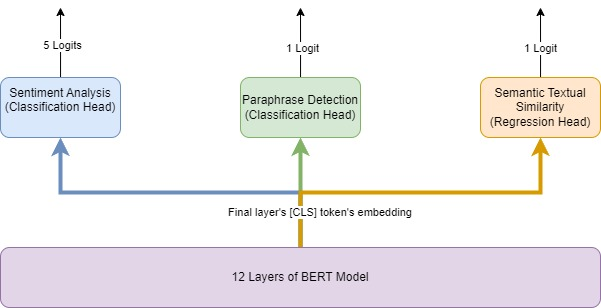
\includegraphics[width=90mm]{Figures/Proposed_Model.jpg}
\caption{Proposed Model\label{PM}}
\end{figure}
\section{Project Description}

\subsection{Data}
% \begin{itemize}
%   \item \textbf{Stanford Sentiment Treebank (SST) dataset:}
%   For the SST Dataset we have the following splits:
%   \begin{itemize}
%     \item train (8,544 examples)
%     \item dev (1,101 examples)
%     \item test (2,210 examples)
%   \end{itemize}
%   \item \textbf{Quora Dataset:}
%   For the Quora Dataset we have the following splits:
%   \begin{itemize}
%     \item train (283,010 examples)
%     \item dev (40,429 examples)
%     \item test (80,859 examples)
%   \end{itemize}
%   \item \textbf{SemEval STS Benchmark Dataset:}
%   For the  SemEval STS Benchmark Dataset we have the following splits:
%   \begin{itemize}
%     \item train (6,040 examples)
%     \item dev (863 examples)
%     \item test (1,725 examples)
%   \end{itemize}
% \end{itemize}
\begin{table}[H]
\centering
\begin{tabular}{|l|r|r|r|}
\hline
\textbf{Dataset} & \textbf{Train} & \textbf{Dev} & \textbf{Test} \\
\hline
Stanford Sentiment Treebank (SST) & 8,544 & 1,101 & 2,210 \\
\hline
Quora Question Pairs & 283,010 & 40,429 & 80,859 \\
\hline
SemEval STS Benchmark & 6,040 & 863 & 1,725 \\
\hline
SNLI & 	550,152 & Not used & Not used \\
\hline
\end{tabular}
\caption{Dataset splits used for training, validation, and testing.}
\label{tab:dataset_splits}
\end{table}

\subsection{Baseline}

We define the following baseline to estimate the upper-bound performance achievable with task-specific optimization:

\begin{itemize}
    \item \textbf{Individually fine-tuned BERT models}: Train separate BERT models, each optimized for a single task. This setup serves as a task-specific upper-bound reference using the techniques employed.
\end{itemize}


% We define the following steps to establish our experimental baselines:

% % \item \textbf{Evaluate a simple BERT model} on the three downstream tasks independently to understand baseline performance without techniques applied.

% \begin{enumerate}
%     \item \textbf{Train separately fine-tuned BERT models}, each optimized for a single task, to estimate the maximum performance achievable with the techniques used.
%     % \item \textbf{Fine-tune single BERT model} for all three tasks with task-specific output heads. We gradually apply techniques. First we use the SBERT Architecture only. Then we use SBERT Architecture and apply SMART technique as well. Then SMART SBEWRT with SimCSE. We select model with best accuracy. 
% \end{enumerate}
% % \item \textbf{Evaluate performance after integrating each advanced technique}—SMART, Contrastive Learning, and Siamese SBERT—into the multi-task setup, assessing the impact of these techniques.

\subsection{Evaluation}
We evaluate our approach on three benchmark NLP tasks:
\begin{table}[H]
    \centering
    \begin{tabular}{|c|c|}
    \hline
    \textbf{Task} & \textbf{Evaluation Metric} \\
    \hline
    \textbf{Paraphrase Detection (QQP)} & Accuracy \\
    \hline
    \textbf{Semantic Textual Similarity (STS-B)} & Pearson correlation coefficient \\
    \hline
    \textbf{Sentiment Analysis (SST-5)} & Accuracy \\
    \hline
    \end{tabular}
    \caption{Evaluation metrics for the tasks}
    \label{tasks_ratings0}
\end{table}